\documentclass[11pt]{article}

\usepackage{fullpage}
\usepackage[round,semicolon]{natbib}
\usepackage{amsfonts}
\usepackage{amsmath}
\usepackage{amssymb}
\usepackage{bm}
\usepackage{bbm}
\usepackage{booktabs}
\usepackage[font=footnotesize,labelfont=bf]{caption}
\usepackage{colortbl}
\usepackage{fixltx2e}
\usepackage{float}
\usepackage{graphicx}
\usepackage[hidelinks]{hyperref}
\usepackage[utf8]{inputenc}
\usepackage{natbib}
\usepackage{standalone}
\usepackage[normalem]{ulem}
\usepackage[usenames,dvipsnames,svgnames,table]{xcolor}

\usepackage{indentfirst}
\newcommand{\pr}{\text{Pr}}

\newcommand{\ETAL}{\textit{et al.}}
\newcommand{\EG}{\textit{e.g.}}
\newcommand{\IE}{\textit{i.e.}}
\newcommand{\CF}{\textit{c.f.}}

\usepackage{hyperref}

% NOTE: one sentence per line for nice git diffs
% WD: I'm a fan of source comments like this, instead of the colory ones in the pdf. But Ok fine, have it your way!
\usepackage{color}
% Will comments
\newcommand{\wdcomment}[1]{{\color{magenta}{(\textbf{WD's comment:} #1)}}}
% Andy comments
\newcommand{\amcomment}[1]{{\color{blue}{(\textbf{AM's comment:} #1)}}}
% Sarah comments
\newcommand{\skhcomment}[1]{{\color{red}{(\textbf{SH's comment:} #1)}}}


\title{Phyload: a story of paired sites finding their way in an unpaired model space}

% WD: this alphabetical author list is copied from the previous version, not meant to indicate priority
\author{
William DeWitt$^{1\ast}$, Sarah Hilton$^{1\ast}$, and Andrew Magee$^{2\ast}$\\
\small{Departments of $^1$Genome Sciences and $^2$Biology, University of Washington, Seattle, USA}\\
\small{$^\ast$ Equal contribution}
}
% \author[1]{Sarah Hilton}
% \author[2]{Andy Magee}

% \affil[1]{Department of Genome Sciences, University of Washington, Seattle, USA}
% \affil[2]{Department of Biology, University of Washington, Seattle, USA}

\begin{document}

\maketitle

\amcomment{We should take the time to consider clearing up our nomenclature. Sites, site pairs, epistatic sites, iid sites, all of these are things that could easily get us into trouble when writing/communicating our results to people.}

\begin{abstract}
Phylogenetic inference relies on probabilistic models of character state change along tree branches in which sites in the alignment are statistically independent.
This severely restrictive assumption facilitates computational tractability, but cannot accommodate epistatic coupling of sites during the evolution of functional sequences that arise from structural and functional constraints on the encoded molecule.
We consider the effect of this misspecification error on the accuracy of phylogenetic reconstruction in a setting of pairwise epistasis.
We show that including epistatically coupled sites in an alignment improves reconstruction accuracy and we introduce an alignment test statistic that is diagnostic for epistasis and can be used in poster predictive checks.
\end{abstract}

\section*{{Introduction}\label{sec:intro}}

Epistasis is $<$definition$>$
This phenomenon is pervasive in datasets for phylogenetic inference $<$citations$>$

Phylogenetic models of epistasis have a long history... we should be sure to emphasize here that most of these are pair models.
$<$We need to talk up the NH model here a decent bit$>$
\amcomment{We also need to be clear if we're going to discuss it as a model that has both iid and interacting sites or not, so we can be clear about our terminology when we set up our grid}

However, phylogenetic models of epistasis are not without drawbacks.
When applying these models in practice, most require that a user specify \textit{a priori} all pairs of sites that are interacting $<$cite doublet models, NH model, pre-RJ Salamin models, others if we come across them$>$.
In some cases such as identifying pairs of stem sites in ribosomal RNA (rRNA), this is possible, if difficult $<$citations on the shitshow of annotating things? maybe some of the databases?$>$.
Even these models of epistasis are more computationally demanding than models that assume all sites are iid by increasing the size of the rate matrix from $4 \times 4$ to $16 \times 16$ and thus
Nonetheless, in many cases there is no hope for pre-defining pairs of interacting sites, which lead \cite{meyer2019simultaneous} to develop a suitable extension of epistatic models for the case where interacting sites must be inferred.
The cost of their approach is that the dimensionality of the parameter space is both drastically increased and variable, requiring reversible-jump MCMC \citep{green1995reversible} to sample from the posterior distribution of the assignments of sites to interacting pairs.

In parallel to the literature on phylogenetic models of epistasis, a literature on detecting epistasis in phylogenetic datasets.
$<$Citations and some literature reviewing$>$
Something something but this literature has mostly been confined to detecting the presence of epistatic interactions in datasets, and decoupled from either modeling these interactions or asking whether they exert a notable effect on phylogenetic inference.
Mumble mumble they should have been doing posterior-predictive testing, or at least using alignment-based summary statistics because those are better because reasons.

Given the difficulties involved in applying epistatic phylogenetic models to real datasets, whether broadly applicable \citep{meyer2019simultaneous} or more specific to the dataset at hand $<$doublet and NH citations$>$, we seek to answer three questions involving the use of misspecified (site-iid) models for dataset where epistasis exists.
First and foremost, what is the effect of including epistatically paired sites in inference?
Secondly, can we detect the presence of epistatic interactions in datasets using posterior-predictive simulations?
Thirdly, is there a test-statistic or set of test-statistics that allow researchers to detect the presence of specifically problematic epistasis?
That is, if there is epistasis in a dataset and failing to model is is causing poor or inadequate phylogenetic inference, is there a way to know we are in this regime?

To address these questions, we perform a simulation study using the epistatic model of \cite{nasrallah2013phylogenetic}, which has a single parameter, $d$ that controls the strength of epistatic interactions.
We simulate alignments on a 3-dimensional grid, defined by the number of sites in the alignment that site-iid, the number of sites(not site-pairs) that are drawn from a paired model, and the value of $d$.
Our grid thus includes a variety of alignment sizes.
This allows us to answer our first question and determine whether the inclusion of epistatic sites in an alignment improves or worsens phylogenetic estimates by tracing a line (for a fixed value of $d$) of increasing numbers of epistatic sites for a fixed value of iid sites.
We define a set of test statistics, including several new ones designed to pick up on patterns of epistasis, and several previously described more general test statistics.
By comparing across levels of epistasis in our simulated alignments, and by their use in posterior predictive checks, we address whether epistasis can be detected directly from alignments, answering our second question.
By combining the posterior-predictive analyses used to answer question 2 and the accuracy results used to answer question 1, we can address whether we can detect problematic epistasis, answering our third question.




Specifically, we ask if epistatic sites are useful but simply not as informative as independent sites or if they are actively harmful to inference.
In other words: does the model misspecification grossly
% \amcomment{That Huelsenbeck ``effective alignment length'' paper may sort of preclude the idea that these sites are actively harmful, but if we want to sell this work as a useful general framework it's worth pointing out you could get at that with this approach.}


Look at all the dumb shit physics/math/CS people have been saying about inferring phylogenies being impossible because selection.
Will's pal (who will remain unnamed) deigned to opine, but upon further discussion revealed that he doesn't know what a codon is, or a synonymous mutation.
We will crush them.

It would be nice to write an intro to phylo modeling that builds up complexity, mentioning GTR+$\Gamma$ and ExpCMs, then the \cite{nasrallah2013phylogenetic} stuff.

\section*{Methods\label{sec:methods}}

\begin{figure}
  \centering
  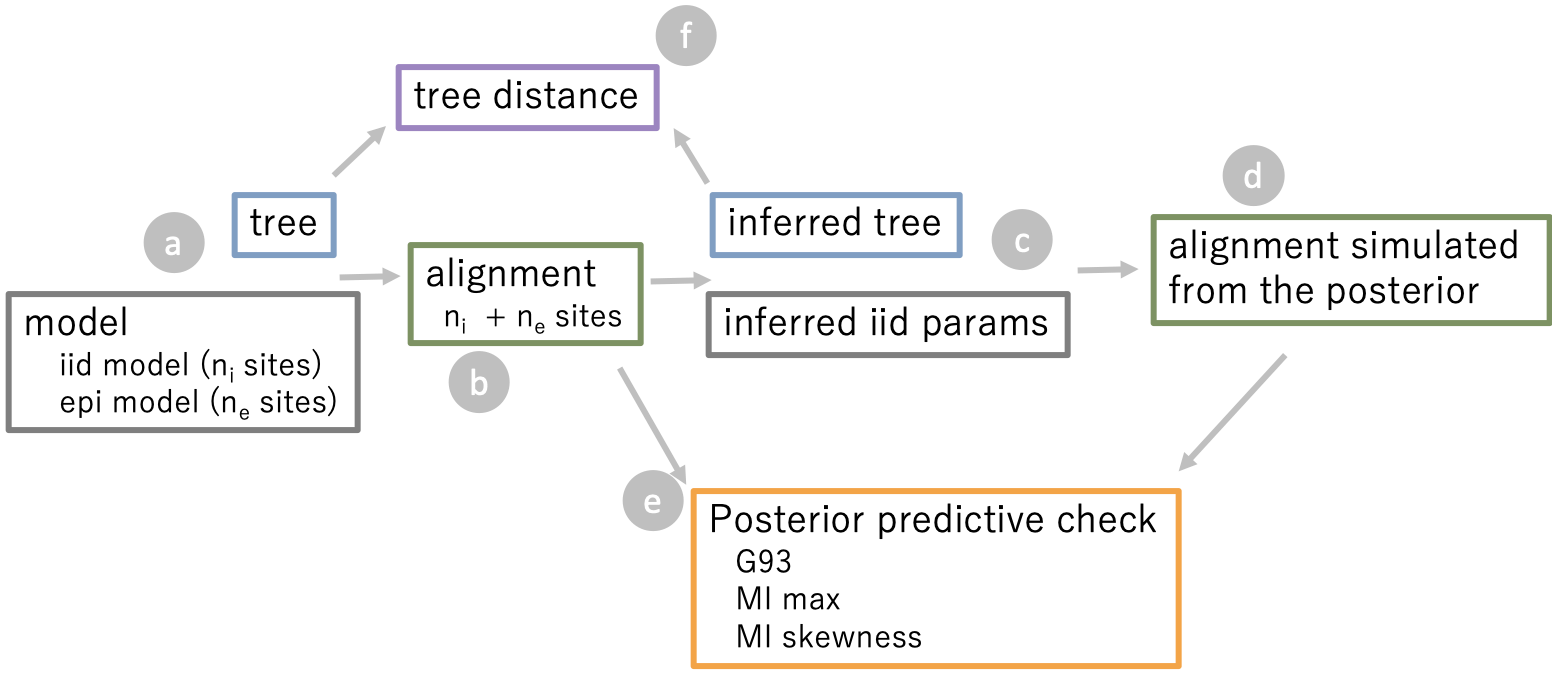
\includegraphics[width=\textwidth]{figures/schematic.png}
  \caption{
a) Tunicate tree, iid model and epi model fit to tunicates. b) simulate alignments under the models in (a). These simulated alignments vary in their lengths, proportion of epistatic sites, and strength of the epistatic interactions. c) MCMC on the simulated alignments. d) simulate alignments from the posterior of (c). e) posterior predictive check using either the G93 metric, MI max or MI skewness. f) RF distance between true tree and inferred tree. 
  }
  \label{fig:schematic}
\end{figure}

\subsection*{Model\label{sec:model}}

\amcomment{We should change this around in an order we like and with notation we like.}

For all our simulations, we employ the epistatic RNA doublet model of \cite{nasrallah2013phylogenetic}, which we implemented in RevBayes \citep{hohna2016revbayes}.
In this model, there are two categories of sites: paired sites experiencing epistatic interactions (which we will refer to as epistatic sites) and unpaired sites evolving independently (which we will refer to as independent sites).
Within each category, it is assumed that all sites (or site pairs) evolve under the same model.
The independent sites evolve under a standard GTR+G substitution model \citep{tavare1986some}.
The epistatic sites evolve under a generalization of the RNA doublet model of \cite{schoniger1994stochastic} with gamma-distributed rate heterogeneity.
The (symmetric) nucleotide exchange rates and the shape parameter of the gamma-distributed rate heterogeneity are shared between the models for the independent and epistatic sites.
We now describe the model for epistatic sites.

Let $\boldsymbol{Q}$ be the instantaneous rate matrix describing changes from doublet $\boldsymbol{x}$ to doublet $y$.
For $\boldsymbol{x} = (x_1, x_2)$, $x_1$ is the 5' nucleotide and $x_2$ is the 3' nucleotide.
The rate matrix is defined as,
\begin{equation}
\label{eq:Q}
\boldsymbol{Q} = \xi \times
\begin{cases}
   \pi_{y} S_{x_1, y_1} & \mbox{if single substitution at the 5' site,} \\
   \pi_{y} S_{x_2, y_2} & \mbox{if single substitution at the 3' site,} \\
   \pi_{y} S_{x_1, y_1} S_{x_2, y_2} d & \mbox{if double substitution where ${\boldsymbol{x}}$ and ${y}$ $\in {\boldsymbol{W}}$,} \\
   0 & \mbox{if any other double substitution,} \\
   - \sum_{\boldsymbol{x} \ne y} Q_{\boldsymbol{x},y}& \mbox{if $\boldsymbol{x}$ = $y$} \\
   \end{cases}
\end{equation}
where $\boldsymbol{S}$ is the GTR exchangeability matrix (shared with the independent sites) and $S_{x_i,y_i}$ is understood to be the element in $S$ governing the rate of exchangeability between nucleotide $x_i$ and $y_i$ (by definition, $S_{x_i,y_i} = S_{y_i,x_i}$),
${\boldsymbol{W}} = (AT, CG, GC, TA)$ is the set of Watson-Crick pairs,
$\boldsymbol{\pi} = (\pi_{AA}, \pi_{AC}, ..., \pi_{TT})$ are the stationary state frequencies of the 16 possible doublet states,
$d$ controls rate of double to single mutations between doublets,
and $\xi$ is the rate-scaling factor (the matrix is normalized to one substitution per single site for comparability with the independent sites).

The parameter $d$ controls the strength of epistatic interactions.
At $d = 0$, there are no double substitutions and this model collapses to the model of \cite{schoniger1994stochastic}.
When $d = \infty$, all substitutions are double substitutions.
In the intervening regimes, a portion of substitutions at epistatically paired sites will be doublet substitutions while the remainder will be single-site changes.
We can compute the total fraction of the substitutions that are doublet substitutions as,
\[
p = \frac{ d \times r_{d} }{d \times r_{d} + r_{s}}
\]
with $r_d$ $1 / d$ times the total rate of doublet subtitutions,
\[
  r_{d} = \sum_{x,y \in \boldsymbol{W}} \pi_{xy} \pi_{yx} S_{x_1,y_1} S_{x_2,y_2},
\]
and $r_s$ the total rate of single substitutions,
\[
  r_{s} = \sum_{x,y \not\in \boldsymbol{W}} \pi_{xy} \pi_{yx} S_{x_1,y_1} S_{x_2,y_2}.
\]
It can thus be seen that (for fixed values of other substitution parameters) the proportion of doublet mutations is a strictly increasing, sigmoidal, function of $d$.
In the case of $d = 0$ and $\pi_{xy} = \pi_x \pi_y$, the model collapses to a standard GTR+G model.

\subsection*{Simulation\label{sec:simulation}}

\subsubsection*{Simulation grid\label{sec:leviathan}}
With the epistatic doublet model, there are two variables that govern the capacity for epistasis to affect phylogenetic inference: the strength of the interactions, and the proportion of the alignment that is epistatic.
To investigate the effect of the strength of epistasis, we simulate with $d = \{0.0,0.5,2.0,8.0,1000.0\}$, which encompasses both realistic (see below) and extreme values.
Simulating $d=0$ allows us to disentangle the effect of model misspecification due to the doublet stationary frequencies from model misspecification due to paired substitutions.
Our values of $d$ correspond to 0\%, 3.2\%, 11.6\%, 34.5\%, and 98.5\% of all substitutions being doublet substitutions.
\skhcomment{All substitutions at epi pairs are doublets, not all subs across the tree, yes?}
To understand the effect of adding epistatic sites, for each value of $d$ we simulate a grid where we independently vary the number of epistatic sites, $n_e$ and independent sites, $n_i$.
This setup is more informative than a one in which we hold the number of sites constant and vary the proportion of sites coming from the epistatic model.
By comparing the accuracy of inference on a dataset with $n_i$ independent sites and one with $n_i$ independent sites and $n_e$ epistatic sites, we can determine if we are in the catastrophic model misspecification regime (inference with $n = n_i + n_e$ sites is worse than with $n = n_i$ sites) or the best-case regime (inference with $n = n_i + n_e$ is better than with $n = n_i$ sites).
\skhcomment{I like the idea of being very clear here what the possible outcomes are. Andy mentioned in slack that we want to be clear that we think epi sites are less useful but not misleading.}

For each value of $d$, we simulate a grid with $n_i,n_e \in \{0, 16, 32, \dots, 400\}$, excluding the cell in which $n_i = n_e = 0$.
To keep computation costs down, at each grid point we simulate a single alignment, and we refer to these alignments collectively as the ``real'' alignments.
While this setup does not afford us a precise estimtate of any quantity at any grid cell, this is not an issue.
For our statistical analyses, including estimation of the value of an epistatic site, the presence of sampling noise is expected by the models.

\subsubsection*{Simulating parameters\label{sec:tunicates}}
To ensure that our simulation regime is realistic, we targeted our simulating parameters on values inferred from the dataset of \cite{tsagkogeorga2009updated}.
As we are primarily interested in the epistatic model parameters, we first inferred a fixed tree using RAxML \citep{stamatakis2014raxml}.
Fixing this tree, we then used RevBayes \cite{hohna2016revbayes} to infer the epistatic doublet model parameters.
The inferred value of $d$ for this dataset is approximately 0.65, while Nasrallah and Huelsenbeck inferred values as high as 7.59 in fixed-tree analyses and 9.72 when inferring the tree.
\skhcomment{N+H used a different tree right? We don't expect to the same value as they did but we expect to get order of magnitude close?}
Thus, our simulating values of $d$ include both extreme values, $d=\{0,1000\}$, and biologically relevant values, $d = \{0.5,2.0,8.0\}$ as biologically relevant values, with the inclu $d=\{0,1000\})$.
We use the RAxML tree for simulation, and all other parameters are fixed to the posterior mean values from the RevBayes analysis.
Simulating values of all parameters are available in Supplementary Table \ref{}.

\subsubsection*{Bayesian inference\label{sec:mcmc}}
We use RevBayes \citep{hohna2016revbayes} to infer unrooted phylogenies for each of the ``real'' alignments.
In all cases, we use a single GTR+G substitution model, intentionally ignoring the presence of epistasis in the datasets.
Details of the model setup, priors, and MCMC moves used are available in the supplement.
For each analysis we run two independent MCMC chains.
In order to avoid analysis artifacts due to convergence issues we perform convergence diagnostics and exclude all grid cells that fail from downstream analysis.
As we are interested in the phylogeny specifically, our convergence diagnostics focus on the tree and branch lengths.
First, we use the average standard deviation of split frequencies (ASDSF) to compare topologies between the two chains.
To account for the possibility of branch-length convergence issues, we also check if the tree length distributions between chains by using the potential scale reduction factor \citep[PSRF,\ ][]{brooks1998general}.
We discard all chains where either ASDSF $>$ XXX or PSRF $>$ YYY.


\subsection*{Posterior predictive assessments\label{sec:pps}}

The posterior-predictive distribution is the distribution on new (replicate) datasets, $y^{\text{rep}}$, that we could draw from our posterior distribution, $p(\theta \mid y)$.
It is obtained by integrating the probability of a new dataset given a particular value of the model parameters $p(y^{\text{rep}} \mid y, \theta)$, across the posterior,
\[
  p(y^{\text{rep}} \mid y) =
  \int p(y^{\text{rep}} \mid y, \theta)\,
  p(\theta \mid y)\,
  \text{d}\theta.
\]
Often we are more interested in a particular feature of a dataset, given by a test statistic $T(y)$.
The posterior predictive distribution for this test statistic is given by,
\[
  p(T(y^{\text{rep}}) \mid y) =
  \int p(T(y^{\text{rep}}) \mid y, \theta)\,
  p(\theta \mid y)\,
  \text{d}\theta.
\]
We can use the posterior predictive distribution of a test statistic to determine if our model is adequate, or in other words if it fits the data in the absolute sense.
If the model is adequate, than the observed value of the test statistic on the real data, $T(y)$, should be near the center of mass of the posterior predictive distribution and not out in the tails.
We can thus compute a posterior predictive p-value, $\text{Pr}(T(y^{\text{rep}}) \geq T(y))$, and if the posterior-predictive p-value is smaller than some threshold $\alpha$, we declare the model to be inadequate.
In practice, one obtains a Monte Carlo estimate of the posterior predictive p-value by simulating new datasets using the draws from the posterior obtained by MCMC, computing the test statistic for each, and calculating the proportion greater than or equal to the observed value.
For a more complete introduction to posterior predictive model checks see \citet{gelman2004bda}, or for a review of model adequacy in evolutionary biology see \citet{brown2018evaluating}.

One of our key questions is, can the presence of unmodeled epistatic interactions be detected with posterior predictive checks?
A test statistic should be chosen on the basis of its ability to detect a particular form of model variation.
As epistasis has yet to be studied from a posterior predictive perspective, there are currently no test posterior predictive approaches designed explicitly to detect it.
We first examine whether a standard phylogenetic posterior predictive test-statistic, the multinomial likelihood test statistic of \cite{goldman1993statistical} can detect this model misspecification.
We then develop two new statistics based on information theory that directly address the expected behavior of epistasis.

We will examine the performance of these test statistics on simulated datasets in two ways.
First, by using only the simulated ``real'' alignments, we will examine if these test statistics are sensitive in principle to the presence of epistasis and to the proportion of epistatic sites in the alignment.
A test statistic that is sensitive in principle to epistatic interactions among sites should vary with the proportion of epistatic sites in an alignment and/or with $d$.
Then we will perform posterior predictive checks for all inferred phylogenies to determine if the statistics are able to detect epistasis in practice.
As an example of this distinction, consider that in principle the GY statistic is capable of detecting the difference between certain GTR \citep{tavare1986some} models and certain HKY \citep{hasegawa1985dating} models.
However, if we simulate an alignment under HKY and infer it under GTR, we will not see any evidence of misspecification \citep{bollback2002bayesian}, so in practice it cannot detect all forms of misspecification.

\subsubsection*{Multinomial likelihood\label{sec:goldman}}

The multinomial likelihood test statistic treats the multiple sequence alignment $\boldsymbol{D}$ as a draw from a multinomial distribution on all possible site patterns.
For $t$ taxa and a DNA or RNA alignment, there are $4^t$ such patterns, and for an alignment of length $n$ we observe some number $s \leq n$ site patterns.
If $s_i$ is the number of times we see site pattern $i$, the maximum likelihood estimate of the multinomial probability of seeing pattern $i$ is $p(i) = s_i / n$.
The test statistic is simply the log-likelihood of this dataset using these estimated probabilities, or $\mathcal{L} = \sum_i [ s_i \log(s_i)]  - n \log(n)$.

\subsubsection*{Mutual information\label{sec:mi}}

Under a phylogenetic model, all sites are conditionally independent given the phylogeny.
However, under the epistatic doublet model, epistatic pairs of sites evolve dependently along the phylogeny due to both $d$ and the use of doublet stationary frequencies.
In particular, the presence doublet substitutions make it more likely that when one site in a pair changes along a branch, the other site does as well.
This should result in pairs of epistatic sites having more similar patterns than independent sites, and the degree of this similarity should depend on $d$.
What is needed, then, is a way to capture this idea of the similarity of sites.

Mutual information is a measure of the dependency of two variables, quantifying the amount of information that one contains about the other.
The higher the mutual information, the more that knowing the value of one variable tells you about the other, in other words the more similar the two variables are.
As above, we assume that we have an $t$ taxa by $n$ sites multiple sequence alignment $\boldsymbol{D}$, and here we denote the alphabet of this alignment $\mathcal{A}$.
For an RNA alignment, $\mathcal{A} = (A,C,G,U)$, for a DNA alignment, $\mathcal{A} = (A,C,G,T)$.
The mutual information of a pair of sites $(i,j)$ is given by,
\[
I_{ij} = \sum_{(a,b)\in\mathcal{A}^2}f_{ij}(a,b)\log\left(\frac{f_{ij}(a,b)}{f_i(a)f_j(b)}\right),
\]
where $f_i(a)$ is the relative frequency of character $a$ at site $i$,
\[
f_i(a) = \frac{1}{t}\sum_{k=1}^{t}\mathbbm{1}_{\{D_{ki}\}}(a),
\]
and $f_{ij}(a,b)$ is the relative joint frequency of character $a$ at site $i$ and character $b$ at site $j$,
\[
f_{ij}(a,b) = \frac{1}{t}\sum_{k=1}^{t}\mathbbm{1}_{\{D_{ki}\}}(a) \mathbbm{1}_{\{D_{kj}\}}(b).
\]

If we had an \textit{a priori} hypothesis about a pair of interacting sites $(i,j)$, we could thus compute the posterior predictive distribution of $I_{ij}$ and compare the observed value to this distribution.
However, if one wants to test for the presence or absence at the level of the entire alignment, this will not work.
However, for an alignment we can compute the mutual information of all pairs of sites, $\boldsymbol{I}$.
As we expect epistasis to increase the mutual information between pairs of interacting sites, the upper tail of $\boldsymbol{I}$ should be informative with respect to the overall presence and strength of epistasis.
We consider two summaries of $\boldsymbol{I}$.
First we consider the skew of $\boldsymbol{I}$, $I_s$, which should be sensitive to the strength of epistasis and proportion of epistatic sites, as the more interactions the more values that should fall in the right tail and the stronger the interactions the larger those values should get.
We also consider the max, $I_m$, which should be sensitive to the presence or absence of epistasis, but is less likely to be sensistive to the proportion of epistatic sites.

\subsection*{Data and code availability\label{sec:its_on_github}}
All the code you need to reproduce these analyses is available somewhere.
But not all the files we produced because that's a loooot of logfiles and a loooot of space required, sorry.

\section*{Results\label{sec:results}}

\subsection*{Accuracy\label{sec:error}}
Preamble preamble preamble.

\subsubsection*{Posterior measures\label{sec:tree_dists}}
As we are interested in Bayesian inference, we are not primarily interested in the error in point estimates of the phylogeny but in the overall goodness of the posterior distribution of trees.
We employ two tree distance metrics, the Robinson-Foulds (RF) distance \citep{robinson1981comparison} and the branch score or Kuhner-Felsenstein (KF) distance \citep{kuhner1994simulation}.
RF distance is a purely topological measure between a pair of trees, capturing the number of splits (bipartitions of taxa) present in one tree but not in the other.
The KF distance is the sum of squared differences in branch lengths between trees, treating a missing split in either tree as a 0, and so captures differences in both topology and branch length.
We compute the posterior distribution of the distance between each tree in the posterior and the true tree using both the KF and RF distances.
We then summarize these distributions by recording the mean, median, min, and max of the distances, as well as the 2.5, 5, 95, and 97.5 percentiles.

As both $d$ and the proportion of epistatic sites increase, so does the distance between the true tree and the posterior as measured by the average posterior KF distance.
However, the addition of epistatic sites improves rather than worsens inference, meaning the catastrophic model misspecification scenario does not apply.
We find that overall the pattern is the same for both the KF and RF distances and for different summaries of the posterior distribution on distances.
Thus we present only the results for the posterior mean KF distance in Figure \ref{fig:rf_mean}, additional results are available somewhere but maybe not in the supplement because that's 15 figures right there.

\begin{figure}
  \centering
  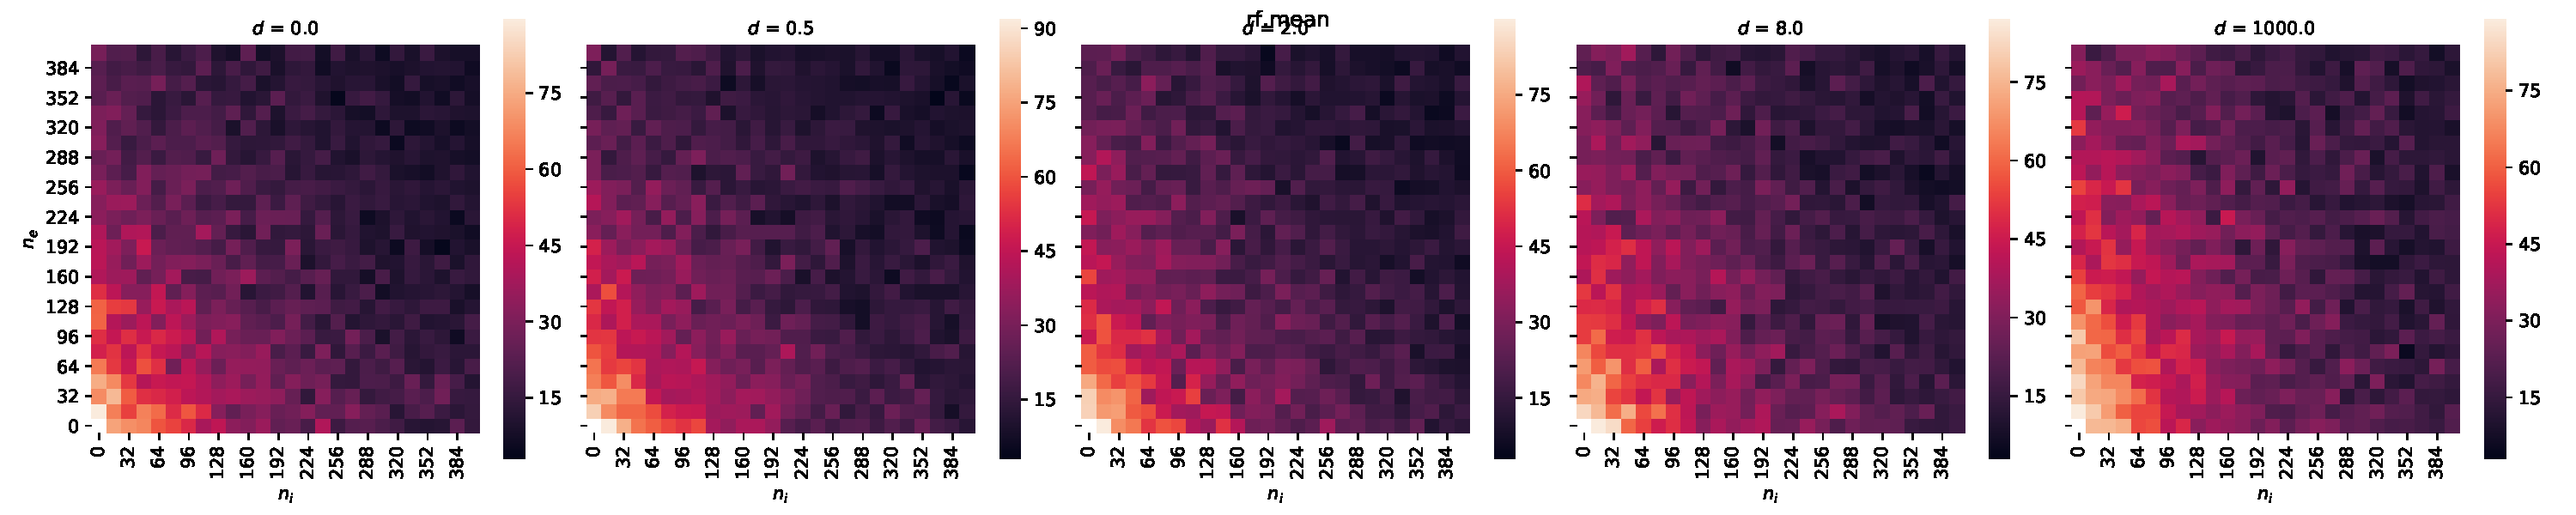
\includegraphics[width=\textwidth]{figures/agg_rf_mean.pdf}
  \caption{
  The posterior mean RF distance to the true tree, plotted as a heatmap.
  Larger values represent posterior distributions that are further on average from the true tree.
  }
  \label{fig:rf_mean}
\end{figure}

\subsubsection*{Summary trees\label{sec:point_estimates}}
While comparisons based on the entire posterior distribution are useful for understanding the overall performance of inference, they do not necessarily reflect the experience of practitioners inferring phylogenies.
In practice, the posterior distribution is, at least for the purposes of visualization, generally reduced to a single summary tree, often a majoriy rule consensus (MRC) tree.
Thus, as an alternative measure of inference error, we look at the number of splits in the MRC tree that are not in the true tree.
The results here largely recapitulate those based on the entire posterior distribution: epistatic sites improve inference, but not as much as an equal number of independent sites, and as $d$ increases their relative utility decreases.

\subsection*{Precision\label{sec:variance}}
We lastly investigated the effect of epistatic interactions on the variance of the posterior distribution on phylogenies.
Intuitively one would expect that if epistasic sites are simply less informative than independent sites, the variance of the posterior distribution on trees should increase.
While the variance of a phylogeny is defined \citep[e.g.\ ][]{willis2019confidence}, the time required to compute this variance makes it prohibitively expensive for our purposes \citep{brown2019mean}.
In order to address the matter of variance, we thus turn to two surrogates.

\subsubsection*{Tree distances\label{sec:kf_variance}}
The first metric we consider is the width of the 95\% CI of the distance to the true tree.
The less information there is in an alignment, the smaller the peak of this distribution one would expect at low values and thus the wider the region spanned by a 95\% CI.
We use our results for the KF distance metric here, as this includes both topological and branch length variation.

As can be seen in Figure \ref{fig:} we were either totally right or completely wrong, so that's cool.

\subsubsection*{Resolution of the summary tree\label{sec:MRC}}
The width of the tree distance distributions is tied in part to the accuracy of the inferred phylogeny, which is not ideal.
We turn now to a measure that is independent of accuracy: the resolution of the majority-rule consensus (MRC) tree \citep{}.
The MRC tree is obtained by including all splits in the posterior that occur with a frequency above 50\%.
As the amount of information in an alignment dwindles, there should be fewer splits with sufficient signal to place in the MRC tree and the MRC tree should include more polytomies.
An MRC tree on $t$ taxa includes a maximum of $2 t - 3$ non-trivial splits, so dividing the number of (non-trivial) splits in the MRC tree by $2 t - 3$ produces a standardized value in [0,1] which we call the proportion of resolved splits.
At 0, the MRC tree is completely unresolved (a star tree), while at 1 it is a fully resolved tree.

We plot the proportion of resolved splits in Figure \ref{fig:}, which shows things and stuff.

\subsection*{Effective sequence length\label{sec:error}}
Given that epistatic sites do not appear to make inference worse, but simply do not provide as much information as independent sites, we sought to quantify this effect.
We use some technique to do this...
\amcomment{We should give some strong consideration to how we want to do this and especially what the most natural scale is for the number of sites and for error.}


\section*{Discussion\label{sec:discussion}}

Phylogenetics is probably fine.

\section*{Supplementary Material}


\section*{Acknowledgments}
We thank our PIs for giving us the freedom to pursue this project and the gods for not striking us down for our unholy combination of python, R, and Rev scripting.

\bibliographystyle{plainnat}
\bibliography{refs}






\end{document}
